%iffalse
\documentclass[journal]{IEEEtran}
\usepackage[a5paper, margin=10mm]{geometry}
%\usepackage{lmodern} % Ensure lmodern is loaded for pdflatex
\usepackage{tfrupee} % Include tfrupee package


\setlength{\headheight}{1cm} % Set the height of the header box
\setlength{\headsep}{0mm}     % Set the distance between the header box and the top of the text


%\usepackage[a5paper, top=10mm, bottom=10mm, left=10mm, right=10mm]{geometry}

%
\usepackage{gvv-book}
\usepackage{gvv}
\setlength{\intextsep}{10pt} % Space between text and floats

\makeindex

\begin{document}
\bibliographystyle{IEEEtran}
\onecolumn
%endif

\title{2011 PH 40-52}
\author{AI24BTECH11031 - Shivram S}
\maketitle
\bigskip

\renewcommand{\thefigure}{\theenumi}
\renewcommand{\thetable}{\theenumi}

\begin{enumerate}
    \item The isospin and the strangeness of $\Omega^-$ baryon are
    \begin{multicols}{4}
        \begin{enumerate}
            \item $1,-3$
            \item $0,-3$
            \item $1,3$
            \item $0,3$
        \end{enumerate}
    \end{multicols}
    
    \item The lifetime of an atomic state is 1 nanosecond. The natural line width of the spectral line in the emission spectrum
    of this state is of the order of
    \begin{multicols}{2}
        \begin{enumerate}
            \item $10^{-10}$ eV
            \item $10^{-9}$ eV
            \item $10^{-6}$ eV
            \item $10^{-4}$ eV
        \end{enumerate}
    \end{multicols}
    
    \item The degeneracy of an excited state of nitrogen atom having electronic configuration
    $1s^22s^22p^23d^1$ is
    \begin{multicols}{4}
        \begin{enumerate}
            \item 6
            \item 10
            \item 15
            \item 150
        \end{enumerate}
    \end{multicols}

    \item The far infrared rotational absorption spectrum of a diatomic molecule shows
    equidistant lines with spacing 20 cm$^{-1}$. The position of the first Stokes line
    in the rotational Raman spectrum of this molecule is
    \begin{multicols}{4}
        \begin{enumerate}
            \item 20 cm$^{-1}$
            \item 40 cm$^{-1}$
            \item 60 cm$^{-1}$
            \item 120 cm$^{-1}$
        \end{enumerate}
    \end{multicols}

    \item A metal with body centered cubic (bcc) structure shows the first (i.e. smallest angle)
    diffraction peak at a Bragg angle of $\theta = 30\degree$. The wavelength of X-ray used is 2.1
    \AA. The volume of the primitive unit cell of the metal is
    \begin{multicols}{4}
        \begin{enumerate}
            \item 26.2 $\brak{\text{\AA}}^3$
            \item 13.1 $\brak{\text{\AA}}^3$
            \item 9.3 $\brak{\text{\AA}}^3$
            \item 4.6 $\brak{\text{\AA}}^3$
        \end{enumerate}
    \end{multicols}

    \item In the following circuit, Tr1 and Tr2 are identical transistors
    having $V_{BE} = 0.7$ V. The current passing through the transistor Tr2 is

    \begin{center}
    \begin{circuitikz}
        \draw (2, 1) node[npn](a) {};
        \draw (5, 2) node[npn](b) {};
        \draw (2.5, 1) node {Tr1};
        \draw (5.5, 2) node {Tr2};
        \draw ($(a)-(0.18,0)$) circle [radius=12pt];
        \draw ($(b)-(0.18,0)$) circle [radius=12pt];
        \draw (b.collector) -- (5, 4) -- (0, 4) to[battery1,l_=+5V] (0, 0) -- (5, 0) -- (b.emitter);
        \draw (a.base) -- (1, 1) -- (1, 2) -- (b.base);
        \draw (a.emitter) -- (2, 0);
        \draw (2, 4) to[R=100 $\Omega$] (a.collector);
    \end{circuitikz}
    \end{center}
    
    \begin{multicols}{4}
        \begin{enumerate}
            \item 57 mA
            \item 50 mA
            \item 48 mA
            \item 43 mA
        \end{enumerate}
    \end{multicols}

    \item The following Boolean expression
    \begin{align*}
    Y = A \cdot \overline{B} \cdot \overline{C} \cdot \overline{D}
    + \overline{A} \cdot B \cdot \overline{C} \cdot D
    + \overline{A} \cdot \overline{B} \cdot \overline{C} \cdot D
    + \overline{A} \cdot \overline{B} \cdot C \cdot D
    + \overline{A} \cdot B \cdot C \cdot D
    + A \cdot \overline{B} \cdot \overline{C} \cdot D
    \end{align*}
    can be simplified to
    \begin{multicols}{2}
        \begin{enumerate}
            \item $\overline{A} \cdot \overline{B} \cdot C + A \cdot \overline{D}$
            \item $\overline{A} \cdot B \cdot \overline{C} + A \cdot \overline{D}$
            \item $A \cdot \overline{B} \cdot \overline{C} + \overline{A} \cdot D$
            \item $A \cdot \overline{B} \cdot C + \overline{A} \cdot D$
        \end{enumerate}
    \end{multicols}

    \item Consider the following circuit.

    \begin{center}
    \begin{circuitikz}[scale=1]
        \draw (3.5, 2) node[op amp, yscale=-1](a) {};
        \draw (0, 4) node[ground] {} (0, 4) to[R=1 $k\Omega$] (2, 4) to[R=4 $k\Omega$] (5, 4) -- (5, 2) to[short, -o] (6, 2);
        \draw (2, 4) -- (2, 2.5) -- (a.+);
        \draw (1.5, 1) node[ground] {} to[short, -o] (1.5, 1) node[left] {$V_{in}$};
        \draw (1.5, 1.5) to[short, o-] (a.-);
        \draw (6, 1) node[ground] {} to[short, -o] (6, 1) node[right] {$V_{out}$};
        \draw (a.down) -- ++(0, 0.5) node[right] {+10 V};
        \draw (a.up) -- ++(0, -0.5) node[right] {-10 V};
        \draw (a.out) -- ++(0.5, 0);
    \end{circuitikz}
    \end{center}

    Which of the following correctly represents the output $V_{out}$ corresponding to the input $V_{in}$?

    \begin{multicols}{2}
        \begin{enumerate}
            \item
            \begin{tikzpicture}[scale=0.75]
                \draw (0, 0) -- (0, 2.4); 
                \draw[->] (0, 1.2) node[left] {$V_{in}$} -- (5, 1.2) node[below] {time};
                \draw[dashed] (0, 1.6) node[left] {+2V} -- (5, 1.6);
                \draw[dashed] (0, 2.2) node[left] {+5V} -- (5, 2.2);
                \draw[dashed] (0, 0.8) node[left] {-2V} -- (5, 0.8);
                \draw[dashed] (0, 0.2) node[left] {-5V} -- (5, 0.2);
                \draw[thick] (0, 0.2) -- (1, 2.2) -- (2, 0.2) -- (3, 2.2) -- (4, 0.2);

                \foreach \i in {0,...,3} {
                    \draw[dotted] (\i+0.3, 2.4) -- (\i+0.3, -2.5);
                    \draw[dotted] (\i+0.7, 2.4) -- (\i+0.7, -2.5);
                }

                \draw (0, -0.1) -- (0, -2.5); 
                \draw[->] (0, -1.3) node[left] {$V_{out}$} -- (5, -1.3) node[below] {time};
                \draw[dashed] (0, -0.2) node[left] {+10V} -- (5, -0.2);
                \draw[dashed] (0, -2.4) node[left] {-10V} -- (5, -2.4);
                \draw[thick] (0, -0.2) -- (0.7, -0.2) -- (0.7, -2.4) -- (1.7, -2.4) -- (1.7, -0.2) -- (2.7, -0.2) -- (2.7, -2.4) -- (3.7, -2.4) -- (3.7, -0.2) -- (5, -0.2);
            \end{tikzpicture}
            \item 
            \begin{tikzpicture}[scale=0.75]
                \draw (0, 0) -- (0, 2.4); 
                \draw[->] (0, 1.2) node[left] {$V_{in}$} -- (5, 1.2) node[below] {time};
                \draw[dashed] (0, 1.6) node[left] {+2V} -- (5, 1.6);
                \draw[dashed] (0, 2.2) node[left] {+5V} -- (5, 2.2);
                \draw[dashed] (0, 0.8) node[left] {-2V} -- (5, 0.8);
                \draw[dashed] (0, 0.2) node[left] {-5V} -- (5, 0.2);
                \draw[thick] (0, 0.2) -- (1, 2.2) -- (2, 0.2) -- (3, 2.2) -- (4, 0.2);

                \foreach \i in {0,...,3} {
                    \draw[dotted] (\i+0.3, 2.4) -- (\i+0.3, -2.5);
                    \draw[dotted] (\i+0.7, 2.4) -- (\i+0.7, -2.5);
                }

                \draw (0, -0.1) -- (0, -2.5); 
                \draw[->] (0, -1.3) node[left] {$V_{out}$} -- (5, -1.3) node[below] {time};
                \draw[dashed] (0, -0.2) node[left] {+10V} -- (5, -0.2);
                \draw[dashed] (0, -2.4) node[left] {-10V} -- (5, -2.4);
                \draw[thick] (0, -0.2) -- (0.3, -0.2) -- (0.3, -2.4) -- (1.3, -2.4) -- (1.3, -0.2) -- (2.3, -0.2) -- (2.3, -2.4) -- (3.3, -2.4) -- (3.3, -0.2) -- (5, -0.2);
            \end{tikzpicture}
        \item
        \begin{tikzpicture}[scale=0.75]
            \draw (0, 0) -- (0, 2.4); 
            \draw[->] (0, 1.2) node[left] {$V_{in}$} -- (5, 1.2) node[below] {time};
            \draw[dashed] (0, 1.6) node[left] {+2V} -- (5, 1.6);
            \draw[dashed] (0, 2.2) node[left] {+5V} -- (5, 2.2);
            \draw[dashed] (0, 0.8) node[left] {-2V} -- (5, 0.8);
            \draw[dashed] (0, 0.2) node[left] {-5V} -- (5, 0.2);
            \draw[thick] (0, 0.2) -- (1, 2.2) -- (2, 0.2) -- (3, 2.2) -- (4, 0.2);

            \foreach \i in {0,...,3} {
                \draw[dotted] (\i+0.3, 2.4) -- (\i+0.3, -2.5);
                \draw[dotted] (\i+0.7, 2.4) -- (\i+0.7, -2.5);
            }

            \draw (0, -0.1) -- (0, -2.5); 
            \draw[->] (0, -1.3) node[left] {$V_{out}$} -- (5, -1.3) node[below] {time};
            \draw[dashed] (0, -0.2) node[left] {+10V} -- (5, -0.2);
            \draw[dashed] (0, -2.4) node[left] {-10V} -- (5, -2.4);
            \draw[thick] (0, -0.2) -- (0.7, -0.2) -- (0.7, -2.4) -- (1.3, -2.4) -- (1.3, -0.2) -- (2.7, -0.2) -- (2.7, -2.4) -- (3.3, -2.4) -- (3.3, -0.2) -- (5, -0.2);
        \end{tikzpicture}
        \item 
        \begin{tikzpicture}[scale=0.75]
            \draw (0, 0) -- (0, 2.4); 
            \draw[->] (0, 1.2) node[left] {$V_{in}$} -- (5, 1.2) node[below] {time};
            \draw[dashed] (0, 1.6) node[left] {+2V} -- (5, 1.6);
            \draw[dashed] (0, 2.2) node[left] {+5V} -- (5, 2.2);
            \draw[dashed] (0, 0.8) node[left] {-2V} -- (5, 0.8);
            \draw[dashed] (0, 0.2) node[left] {-5V} -- (5, 0.2);
            \draw[thick] (0, 0.2) -- (1, 2.2) -- (2, 0.2) -- (3, 2.2) -- (4, 0.2);

            \foreach \i in {0,...,3} {
                \draw[dotted] (\i+0.3, 2.4) -- (\i+0.3, -2.5);
                \draw[dotted] (\i+0.7, 2.4) -- (\i+0.7, -2.5);
            }

            \draw (0, -0.1) -- (0, -2.5); 
            \draw[->] (0, -1.3) node[left] {$V_{out}$} -- (5, -1.3) node[below] {time};
            \draw[dashed] (0, -0.2) node[left] {+10V} -- (5, -0.2);
            \draw[dashed] (0, -2.4) node[left] {-10V} -- (5, -2.4);
            \draw[thick] (0, -0.2) -- (0.3, -0.2) -- (0.3, -2.4) -- (1.7, -2.4) -- (1.7, -0.2) -- (2.3, -0.2) -- (2.3, -2.4) -- (3.7, -2.4) -- (3.7, -0.2) -- (5, -0.2);
        \end{tikzpicture}
        \end{enumerate}
    \end{multicols}

    \textbf{Common Data for Questions 48 and 49}: \\
    Consider a function $f\brak{z} = \frac{z \sin z}{\brak{z - \pi}^2}$ of a complex variable $z$.
    
    \item Which of the following statements is \textbf{TRUE} for the function $f\brak{z}$?
    \begin{enumerate}
        \item $f\brak{z}$ is analytic everywhere in the complex plane
        \item $f\brak{z}$ has a zero at $z = \pi$
        \item $f\brak{z}$ has a pole of order 2 at $z = \pi$
        \item $f\brak{z}$ has a simple pole at $z = \pi$
    \end{enumerate}
    
    \item Consider a counterclockwise circular contour $\abs{z} = 1$ about the origin. The integral
    $\oint f\brak{z} dz$ over this contour is
    \begin{multicols}{4}
        \begin{enumerate}
            \item $-i\pi$
            \item zero
            \item $i\pi$
            \item $2i\pi$
        \end{enumerate}
    \end{multicols}

    \textbf{Common Data for Questions 50 and 51:} \\
    The tight binding energy dispersion $\brak{E-k}$ relation for electrons in a one-dimensional
    array of atoms having lattice constant $a$ and total length $L$ is 
    \begin{align*}    
    E = E_0 - \beta - 2\gamma \cos\brak{ka},
    \end{align*}
    where $E_0$, $\beta$, and $\gamma$ are constants and $k$ is the wave-vector.

    \item The density of states of electrons (including spin degeneracy) in the band is given by
    \begin{multicols}{4}
        \begin{enumerate}
            \item $\frac{L}{\pi \gamma a \sin\brak{ka}}$
            \item $\frac{L}{2\pi \gamma a \sin\brak{ka}}$
            \item $\frac{L}{2\pi \gamma a \cos\brak{ka}}$
            \item $\frac{L}{\pi \gamma a \cos\brak{ka}}$
        \end{enumerate}
    \end{multicols}
    
    \item The effective mass of electrons in the band is given by
    \begin{multicols}{4}
        \begin{enumerate}
            \item $\frac{\hbar^2}{\gamma a^2 \cos\brak{ka}}$
            \item $\frac{\hbar^2}{2\gamma a^2 \cos\brak{ka}}$
            \item $\frac{\hbar^2}{\gamma a^2 \sin\brak{ka}}$
            \item $\frac{\hbar^2}{2\gamma a^2 \sin\brak{ka}}$
        \end{enumerate}
    \end{multicols}
\end{enumerate}
\end{document}
